\section{The pre-existing project}

The census page that contains the data in digital form holds a wealth of information about each person surveyed: name, gender, membership status and some secondary features such as work or the breed. 

All these data are housed in a moulded grid composed of numbered rows and columns. In addition to the citizens data, each archive also contains additional information related to the censor or data relating to samples of the population.

The project's objective was finding a particular grid area, corresponding to the area containing the registered State of each person, from which extract the handwritten text.

Following the words localization, the existing work proceeds by grouping visually similar elements to form a collection of homogeneous samples, in hope that each set will then contain cut outs of the same State.

The goal of the work is not to group all the words corresponding to the same state in a single cluster but rather to generate clusters that contain words that belong to a single state, the major requirement of the work is thus precision in the retrieval steps.

\subsection{Process steps}

We can summarize the project in three basic steps:
\begin{enumerate}
\item Localization of the text area containing the words of interest
\item Row segmentation
\item Post-processing and clustering
\end{enumerate}

The last step, corresponding to the clustering of images, is the point of interest of our paper: while the past work was focused on the localization and retrieval not much thought was put on the features to be extracted preferring simplicity and efficiency to effectiveness.
It is this very point that gives our paper a reason d'etre: starting from the preceding, already implemented, two steps, we proceed by providing a rewritten and improved clustering method through the use of new features, these steps will be discussed later in the section 3.

\subsubsection{Column localization}

In this first phase the aim is to identify the region of the grid within which the State words are located. 

First of all the black border of the document is removed, an artefact resulting from the physical scanning. Then, through a vertical projection of the pixels and the creation of an histogram, the grid columns are located and, knowing the correct column's offset regarding the beginning of the document, just the one concerned is extracted.

\subsubsection{Row segmentation}

After the extraction of the concerned column from the document, we proceed with row segmentation.

Similar to the previous step, but using an horizontal projection this time, we are able to determine with some accuracy the rows of the grid. In this case, however, it's necessary to centre the word in the extracted image: this is done by correcting the height of each row by the analysis of black spikes on the created histogram.

At the end of this phase, ideally each word is contained in an individual image.

\subsubsection{Post-processing and clustering}
\label{oldFeatures}
In the post-processing phase the individual images extracted are reworked in order to remove any  vertical or horizontal residual lines left from an imperfect previous cut.

Delete row/column strokes can be about as bring back the black pixels related to the residual value of pure white (255 as grayscale).

This allows us to extract the most significant features in the next steps of processing.

Each image is divided in windows 1 pixel wide, on these windows the features are then extracted.
The idea is not placing excessive burden on the operating system, the features are thus relatively simplistic: for each window the value of the height of the first and last black pixels are collected, together with the number of transitions of the pixels from black to white and vice versa.
The distance between images is then found through the Euclidean Distance where the considered axis are the number of transitions and the stroke height calculated through a simple subtraction of the first and last black pixels height.
The distance matrix is then fed to the Affinity Propagation algorithm to create the desired clusters.

\begin{figure}[!ht]
\centering
\vspace{0.3cm}
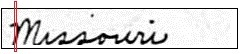
\includegraphics[width=0.5\textwidth]{images/missouri_1pix.jpg}
\caption{An image extracted from document, the red box delineates the 1 pixel wide window.}
\label{fig:extracted_image}
\end{figure}

As you can see in Figure \ref{fig:extracted_image}, the word is centered and the extra line have been removed (there is a line set to white). For each picture we proceed with feature extraction for handwritten characters and clustering. 

\subsection{Problems}

The localization of words and their segmentation has inherent strong difficulties.

A first problem is represented by the document skew. In this case, the skew may be due to a not perfectly horizontal scan of the original document. The presence of skew reduces the capability in searching for rows and columns of the grid, thus making the segmentation impossible with the given implementation. In some cases, for example, the first column is interpreted incorrectly causing the extraction of the wrong column in the first stage of the process thus dooming that particular word recognition.

The main problems of the second phase are mainly related to the identification of extraneous lines. Because of the large number of dashed lines present it isn't always possible to \emph{clean} the images and this can cause errors in the clustering phase.

\begin{figure}[!ht]
 \centering
 \subfigure[An image with a dashed line]
   {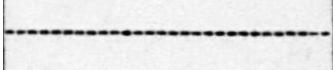
\includegraphics[width=0.3\textwidth]{images/img3.jpg}}
 \hspace{5mm}
 \subfigure[The line intersects the word]
   {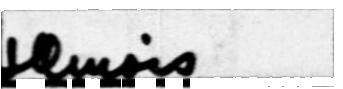
\includegraphics[width=0.3\textwidth]{images/img4.jpg}}
 \caption{Segmentation and post-processing issues}
 \end{figure}

In other cases the word intersects directly gridlines. Because of this we may experience a loss of information about words if the line is removed using the method described above.

